\subsection{Режим счётчика}
\selectlanguage{russian}

Режим счётчика (\langen{Counter, CTR}, рис.~\ref{fig:CTR}) был описан Диффи и Хеллманом в 1979 году.~\cite{Diffie:Hellman:1979} Правило шифрования имеет вид, похожий на режим обратной связи по выходу (OFB), но позволяющий вести независимое (параллельное) шифрование и расшифрование блоков:
\[ \begin{array}{l}
    K_j = E_K(\textrm{Nonce} ~\|~ j - 1), ~ j = 1, 2, \dots, n, \\
    C_j = M_j \oplus K_j,
\end{array} \]
где $\textrm{Nonce} ~\|~ j - 1$ -- конкатенация битовой строки одноразовой метки $\textrm{Nonce}$ и номера блока, уменьшенного на единицу.
%Для стандарта AES значение $\textrm{Nonce}$ занимает 16 бит, номер блока -- 48 бит. С одним ключом выполняется шифрование $2^{48}$ блоков.

\begin{figure}[bt]
	\centering
	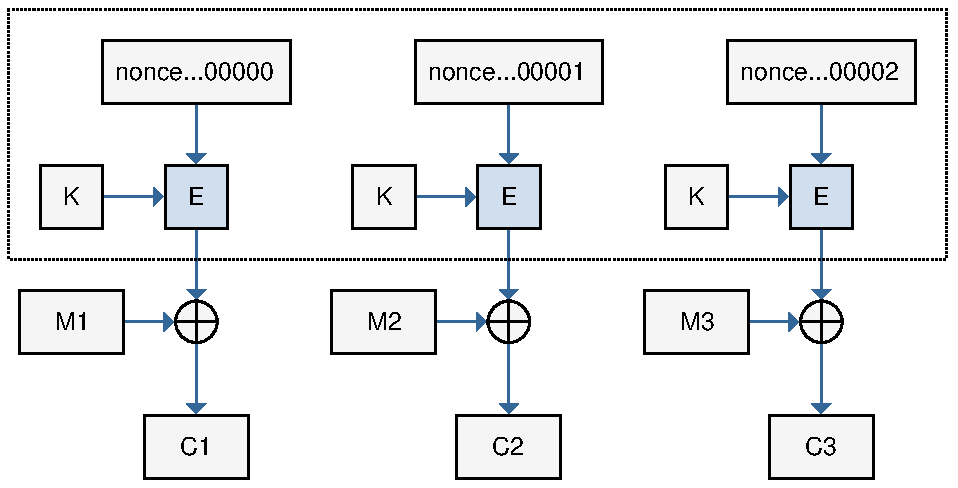
\includegraphics[width=1\textwidth]{pic/CTR}
	\caption{Режим счётчика. Пунктирной рамкой выделена область формирования \emph{гаммы}, независящей от открытого текста.}
	\label{fig:CTR}
\end{figure}

Правило расшифрования идентичное:
\[ \begin{array}{l}
    M_j = C_j \oplus K_j. \\
\end{array} \]

Преимущества:
\begin{itemize}
	\item относительно простая реализация -- операции шифрования и расшифрования совпадают;
	\item нет необходимости дополнять открытый текст до размера, кратного размеру блоку шифрования;
	\item возможность полной параллелизации шифрования (можно приступать к шифрованию любого блока в любой момент);
	\item ошибка передачи одного бита приводит к ошибке в единственном бите открытого текста.
\end{itemize}

Недостатки:
\begin{itemize}
	\item не обеспечивает целостность.
\end{itemize}

В отличии от режима OFB период генерируемой <<гаммы>> всегда одинаков и зависит только от количества бит в \emph{nonce}. Так как после достижения максимального значения счётчика значение \emph{nonce} \emph{не} увеличивается на единицу, период <<гаммы>> равен:
\[
   \textrm{period} = \textrm{size}_\textrm{block} \times 2^{ \textrm{size}_\textrm{block} - \textrm{size}_\textrm{nonce} }.
\]

Данный режим (как и большая часть остальных рассмотренных режимов) обеспечивает только конфиденциальность\index{конфиденциальность} передачи данных, но не целостность\index{целостность}. В модели активного злоумышленника, если последний может предположить о содержимом любой части открытого текста, злоумышленник может поменять отдельные биты шифртекста, что приведёт к предсказуемым (с точки зрения криптоаналитика) изменениям в расшифрованном тексте.